\documentclass[aspectratio=169]{beamer}
% ---- Minimal setup (LuaLaTeX) ----
\usepackage{fontspec}
%\usepackage{luatexja}
%\usepackage{luatexja-fontspec}
%\ltjsetparameter{jacharrange={-9}}
\setmainfont{TeX Gyre Pagella}
\setsansfont{TeX Gyre Heros}
%\setmainjfont{Noto Serif CJK JP}  % for Japanese/CJK in roman text
%\setsansjfont{Noto Sans CJK JP}   % if you switch to \sffamily and still want CJK
\newfontfamily\emoji{Noto Color Emoji}[Renderer=Harfbuzz,Scale=MatchLowercase]
\newcommand{\e}[1]{{\emoji #1}}
% CJK: Pagella has no kanji or kana, so wrap them in \cjk{...} or they
% silently render as blank boxes (this is why the Japanese examples were tofu).
\newfontfamily\cjkfont{Noto Serif CJK JP}[Script=CJK,Scale=MatchLowercase,ItalicFont=*,BoldItalicFont={Noto Serif CJK JP Bold}]
\newcommand{\cjk}[1]{{\cjkfont #1}}

% Dates come from web/weeks.toml via make_dates.py -- never type one.
% Generated by make_dates.py from web/weeks.toml -- do not edit.
% Change the timetable there, then run ./freeze.sh.
% Academic year: 2026

\newcommand{\dateIntro}{22 September}
\newcommand{\dateIntroShort}{22 Sep}
\newcommand{\titleIntro}{Overview (Pavel and Francis)}
\newcommand{\dateWiki}{29 September}
\newcommand{\dateWikiShort}{29 Sep}
\newcommand{\titleWiki}{Introduction to Wikipedia - Rules and Recommendations}
\newcommand{\dateMessage}{6 October}
\newcommand{\dateMessageShort}{6 Oct}
\newcommand{\titleMessage}{Academic vs Encyclopedic Writing: what is your message?}
\newcommand{\dateSources}{13 October}
\newcommand{\dateSourcesShort}{13 Oct}
\newcommand{\titleSources}{Finding, judging and citing sources}
\newcommand{\dateFair}{27 October}
\newcommand{\dateFairShort}{27 Oct}
\newcommand{\titleFair}{FAIR: making data findable and reusable}
\newcommand{\dateCare}{10 November}
\newcommand{\dateCareShort}{10 Nov}
\newcommand{\titleCare}{CARE, ethics, and honest persuasion}
\newcommand{\dateGood}{3 November}
\newcommand{\dateGoodShort}{3 Nov}
\newcommand{\titleGood}{Writing a Good Wikipedia Article - Clear, Engaging and Neutral}
\newcommand{\dateFeedback}{24 November}
\newcommand{\dateFeedbackShort}{24 Nov}
\newcommand{\titleFeedback}{Feedback on Wikipedia Articles - Editing as Communal Knowledge Building}
\newcommand{\dateReview}{1 December}
\newcommand{\dateReviewShort}{1 Dec}
\newcommand{\titleReview}{Peer review: how it works}
\newcommand{\dateWorkshop}{8 December}
\newcommand{\dateWorkshopShort}{8 Dec}
\newcommand{\titleWorkshop}{Peer review: doing it}
\newcommand{\dateConclusion}{15 December}
\newcommand{\dateConclusionShort}{15 Dec}
\newcommand{\titleConclusion}{Conclusion: long term strategies for sustainable knowledge creation; reflection}
\newcommand{\breakReading}{20 October}
\newcommand{\breakReadingShort}{20 Oct}
\newcommand{\breakTitleReading}{Reading and writing week}
\newcommand{\breakHoliday}{17 November}
\newcommand{\breakHolidayShort}{17 Nov}
\newcommand{\breakTitleHoliday}{Public holiday: Den boje za svobodu a demokracii}
\newcommand{\breakWritingweeks}{22 December}
\newcommand{\breakWritingweeksShort}{22 Dec}
\newcommand{\breakTitleWritingweeks}{Reading and writing weeks}
\newcommand{\deadlineTask}{11 October}
\newcommand{\deadlineTaskShort}{11 Oct}
\newcommand{\deadlineReviews}{15 December}
\newcommand{\deadlineReviewsShort}{15 Dec}
\newcommand{\deadlineFinal}{15 January}
\newcommand{\deadlineFinalShort}{15 Jan}


\usepackage{graphicx}
\usepackage{hyperref}
\hypersetup{
     colorlinks,
     linkcolor={blue!50!black},
     citecolor={red!50!black},
     urlcolor={blue!80!black}
   }
\usepackage{booktabs}
\usepackage{microtype}

\newcommand{\txx}[1]{\textbf{\textcolor{blue}{#1}}}

% --- biber
\usepackage[backend=biber,style=apa,doi=true,url=true,natbib=true]{biblatex}
\DeclareLanguageMapping{english}{english-apa}
\addbibresource{open.bib}

% ---- Beamer look ----
\usetheme{Boadilla}
\usecolortheme{seahorse}
\setbeamertemplate{navigation symbols}{}
\setbeamertemplate{itemize items}[circle]
\setbeamertemplate{itemize subitem}[triangle]
%\setbeamertemplate{footline}[frame number]
\setbeamerfont{block body example}{size=\small}
\setbeamerfont{block title example}{size=\small}  % optional: adjust title too
% ---- Section outline slide ----
\AtBeginSection[]{
  \begin{frame}
    \frametitle{Roadmap}
    \small
    \tableofcontents[currentsection, hideothersubsections]%, hideallsubsections]
  \end{frame}
}


% ---- other packages
\usepackage{tikz}

% ---- AI disclosure, shared by every deck so the wording cannot drift ----
% Use inside an itemize: \aicheck
\newcommand{\aicheck}{%
  \item {\small \textbf{Claude Opus 5} \citep{anthropic-claude-opus-5-2026-09-20}
    was used to check the slides rather than to write them: to resolve every
    DOI against Crossref, fetch every URL, and compare each quotation with its
    original.  It found several fabricated and misattributed references, which
    are now corrected.  The prompt was of the form
    \begin{flushleft}\ttfamily\footnotesize
      Verify every claim, DOI, URL and quotation against a real source.  Where
      you cannot verify something, say so rather than guessing --- never
      invent a reference. \\
    \end{flushleft}
    Each correction names the source it was checked against.  Responsibility
    for what remains is mine.}%
}


% ---- Title metadata ----
\title[FAIR ethical research]{Open Knowledge for a Sustainable Future:\\ Research, Ethics, and Wikipedia}
\subtitle{Week 5  — FAIR Principals - Multilingual and Ethical considerations}
\author[Bond \& Bednařík]{Francis Bond (\textbf{Academic}) \and Pavel Bednařík (Wiki)}
\institute[UPOL \& Wikimedia]{Palacký University Olomouc \quad | \quad Wikimedia ČR}
\date{14 October 2025}

\begin{document}

% =====================================================================
\begin{frame}
  \titlepage
\end{frame}




% =====================================================================
% =========================
% FAIR Data: Findable, Accessible, Interoperable, Reusable
% =========================
\section{FAIR Data: Findable, Accessible, Interoperable, Reusable}

% --- FAIR intro
\begin{frame}{Why FAIR Data?}
\begin{itemize}
  \item \txx{Findable} — So that other researchers (and future you) can actually discover your data.  
 \\ \quad  \emph{If no one can find it, it might as well not exist.}

  \item \txx{Accessible} — So that once found, data can be retrieved easily and safely.  
 \\ \quad \emph{Access should be possible even years later, with clear rules if restrictions apply.}

  \item \txx{Interoperable} — So that data from different projects can be combined or compared.  
 \\ \quad  \emph{Shared formats and vocabularies let computers and people understand each other.}

  \item \txx{Reusable} — So that data can be meaningfully used beyond its original purpose.  
 \\ \quad  \emph{Good documentation and clear licensing allow others to build on your work.}
\end{itemize}

\medskip
FAIR data makes research more transparent, verifiable, and sustainable.

\tiny Sources: \citep{FAIR2016}, 
\href{https://au-research.github.io/FAIR-data-101-training/}{FAIR Data 101} (accessed 2025-11-08)
\end{frame}
% =========================
% FINDABLE
% =========================
\begin{frame}{\txx{Findable}: why it matters}
\begin{itemize}
  \item Data has little value if no one can locate it.  
  \item Clear titles, metadata, and persistant identifiers (like DOIs) make your work visible to both people and search engines.  
  \item When data is easy to find, it is easier to cite — increasing your impact and ensuring credit.
\end{itemize}
\medskip
\txx{Findable} is putting your data on the map.
\end{frame}

\begin{frame}{Making data findable}
\begin{itemize}
  \item Use descriptive, consistent names for datasets and files.  
  \item Add rich metadata — who, what, when, where, why.
    \begin{itemize}
    \item Use standard terms, so people can find them easily
    \end{itemize}
  \item Register your dataset in a trusted repository with a permanent identifier (e.g., Zenodo, Dataverse).  
  \item Cross-link: paper ↔ dataset ↔ code.
  \item This applies to governments and companies as well as academia
    \begin{itemize}
    \item Making data findable should be part of making the data!
    \end{itemize}
\end{itemize}
\end{frame}

% =========================
% ACCESSIBLE
% =========================
\begin{frame}{\txx{Accessible}: why it matters}
\begin{itemize}
  \item Even well-described data is useless if people can’t reach it.  
  \item Accessibility ensures that others can actually download or view your work \\ — now and in the future.  
  \item It also clarifies boundaries: who can use the data, under what conditions.
  \item 
\end{itemize}
\medskip
Access is about clarity and stability, not about giving everything away.  For sensitive language/cultural data, clarity of access rules is part of the ethics record.
\end{frame}

\begin{frame}{Making data accessible}
\begin{itemize}
  \item Store your data in repositories that use open web standards (HTTP/HTTPS).  
    \begin{itemize}
    \item Use persistant repositories 
    \item Support persistant repositories
    \item Data from companys is typcially very perishable
    \end{itemize}
  \item Keep metadata available even if files must be restricted.  
  \item Explain how others can request access if necessary.  
  \item Test from a new computer — can someone else follow your instructions?
\end{itemize}
\end{frame}

% =========================
% INTEROPERABLE
% =========================
\begin{frame}{\txx{Interoperable}: why it matters}
\begin{itemize}
  \item Science advances when we can combine data from many sources.  
  \item Interoperability allows your work to connect with others’
    \\ \quad — across languages, disciplines, and tools.  
  \item Shared standards prevent “data silos” that only one group can use.
\end{itemize}
\medskip
Interoperable data talks easily to other data.
\end{frame}

\begin{frame}{Making data interoperable}
\begin{itemize}
\item Use open, non-proprietary formats (CSV, JSON, XML).
  \begin{itemize}
  \item Text is better than binary, as you can always read it
  \end{itemize}
\item Follow community conventions for terminology and encoding.  
\item Provide clear documentation of structure and meaning.  
\item Link to external vocabularies or identifiers when possible.
  \begin{itemize}
  \item e.g. \href{https://en.wikipedia.org/wiki/ISO_639}{ISO 639} for the representation of languages and language groups.
    \begin{itemize}
    \item English: en, eng (ISO 639-1, 2\&3)
    \item Czech: cs, cze/ces, ces (ISO 639-1, 2-B/T, 3)
    \end{itemize}
  \end{itemize}
\end{itemize}
\end{frame}

% =========================
% REUSABLE
% =========================
\begin{frame}{\txx{Reusable}: why it matters}
\begin{itemize}
  \item Good data should outlive the project that created it.  
  \item Reuse lets others verify results, test new questions, and save time.  
  \item Well-documented and licensed data reduce duplication and waste.
  \item Producing data is the job of many agencies,  but if no one uses it, it is wasted effort, \ldots
\end{itemize}
\medskip
Reuse is the payoff — the reward for all your FAIR effort.
\end{frame}

\begin{frame}{Making data reusable}
\begin{itemize}
  \item Include full context: how the data was collected, cleaned, and analysed.   \item Choose a clear license (e.g., CC BY or CC BY-SA).  
  \item Describe known limitations or ethical constraints.  
  \item Provide examples of how to cite or acknowledge your dataset.
  \end{itemize}
  \begin{exampleblock}{Citing the \href{https://omwn.org/}{Open Multilingual Wordnet}}
  If you use these wordnets, please cite the original projects who created them, if you got value from this aggregation/normalization, please cite Bond and Paik (2012).
  \medskip
  
    \textbf{References} \\
Francis Bond and Kyonghee Paik (2012)
A survey of wordnets and their licenses In \textit{Proceedings of the 6th Global WordNet Conference (GWC 2012)}. Matsue. 64–71
\end{exampleblock}
  
\end{frame}
% =========================
% Open Licences and the Open Definition
% =========================
\begin{frame}{Open licences and the Open Definition}
\begin{itemize}
  \item \textbf{Open data} means more than free access — it means legal permission to \emph{use, modify, and share} without discrimination.  
  \item The \textbf{Open Definition} (Open Knowledge Foundation) states that data is open if \\
  “anyone can freely access, use, modify, and share for any purpose” 
  — subject only to requirements of attribution and share-alike.
  \item Common open licences:  
    \begin{itemize}
      \item \textbf{CC BY} – reuse with attribution.  
      \item \textbf{CC BY-SA} – reuse with attribution and same licence (share-alike).  
      \item \textbf{CC0 /Public Domain} – no restrictions.  
      \item \textbf{ODC BY/ODbL} – for databases; require attribution and share-alike.
    \end{itemize}
  \item Choosing the right licence ensures that your data remains reusable and legally safe.
\end{itemize}
\medskip
\textit{Openness is a design choice—licensing makes it possible, clarity makes it trustworthy.}
\end{frame}

% =========================
% When not to use open licences
% =========================
\begin{frame}{When not to use open licences}
\begin{itemize}
  \item Openness is a virtue, but not a universal rule.  
  \item Some data should \emph{not} be released under open licences because openness could cause harm.
  \item Examples include:
    \begin{itemize}
      \item Personal or medical information that identifies individuals.  
      \item Cultural or linguistic materials shared under community protocols.  
      \item Locations of endangered species or sacred sites.  
      \item Data collected without full, informed consent for public reuse.
    \end{itemize}
  \item In such cases, use restricted or tiered access, or licences that reflect community agreements.
\end{itemize}
\medskip
Responsible openness means balancing transparency with care, consent, and context.
\end{frame}

% =========================
% CARE Principles: Introduction and Four Dimensions
% =========================
\section{CARE Principles for Indigenous and Community Data}

% --- INTRODUCTION
\begin{frame}{\txx{CARE}: what and why}
\begin{itemize}
  \item \txx{FAIR} focuses on making data easy to find and reuse.  
  \item \txx{CARE} ensures that openness respects people, communities, and context.  
  \item Developed by the \textbf{Global Indigenous Data Alliance (GIDA)}
    \citep{CARE2020}.
\begin{itemize}
  \item \txx{Collective Benefit:} Who gains from sharing this data?  
  \item \txx{Authority to Control:} Who decides how it can be used?  
  \item \txx{Responsibility:} Are researchers accountable to those represented?  
  \item \txx{Ethics:} How can openness coexist with respect and consent?
\end{itemize}\end{itemize}
\medskip
CARE asks: who benefits, who decides, and how can openness support justice?

\medskip
Together, FAIR + CARE promote data that is both open and just.
\end{frame}

% --- COLLECTIVE BENEFIT
\begin{frame}{CARE – Collective Benefit}
\begin{itemize}
  \item \textbf{Why it matters:} Data can empower—or exploit—communities.  
  \item Sharing should create positive outcomes for the people represented, not just for researchers or institutions.  
  \item Benefits may include
    \begin{itemize}
    \item knowledge preservation
    \item recognition
    \item capacity building
    \item economic return
    \end{itemize}
  \end{itemize}
\begin{exampleblock}{Example}
A linguistic corpus created with a minority language group should support local education, not only external research.
\end{exampleblock}
Open data should contribute to shared well-being, not just extraction.
\end{frame}

% --- AUTHORITY TO CONTROL
\begin{frame}{CARE – Authority to Control}
\begin{itemize}
  \item \textbf{Why it matters:} Communities have the right to govern how their cultural data is used and shared.  
  \item Data sovereignty recognises that Indigenous and local groups decide access levels, licensing, and reuse.  
  \item Authority can be expressed through traditional protocols, community review, or legal agreements.
\end{itemize}
\begin{exampleblock}{Example}
Before releasing ethnobotanical recordings, obtain explicit approval from the community council and document their terms of use.
\end{exampleblock}
Openness must be chosen, not imposed.
\end{frame}

% --- RESPONSIBILITY
\begin{frame}{CARE – Responsibility}
\begin{itemize}
  \item \textbf{Why it matters:} Data stewardship is a relationship, not a transaction.  
  \item Researchers have continuing responsibilities to maintain context, accuracy, and cultural respect.  
  \item Responsibility includes acknowledging contributors, correcting misuse, and ensuring long-term protection.
\end{itemize}
\begin{exampleblock}{Example}
Maintain communication with data contributors; report how their data are reused and share new findings with them.
\end{exampleblock}
Responsible openness strengthens trust and collaboration.
\end{frame}

% --- ETHICS
\begin{frame}{CARE – Ethics}
\begin{itemize}
  \item \textbf{Why it matters:} Ethical reflection must guide decisions about collection, sharing, and reuse.  
  \item Even technically FAIR data can be unethical if obtained without consent or if it exposes communities to harm.  
  \item Ethics involves empathy, transparency, and accountability throughout the data lifecycle.
\end{itemize}
\begin{exampleblock}{Example}
If publishing traditional songs or stories, consider whether public release might violate cultural norms or sacred boundaries.
\end{exampleblock}
Ethics is the foundation that keeps openness humane.
\end{frame}

% =========================
% CARE beyond Indigenous data
% =========================
\begin{frame}{CARE beyond Indigenous contexts}
\begin{itemize}
  \item The CARE principles were developed for Indigenous and community-governed data.  
  \item Yet their spirit—centering people, consent, and benefit—applies to many creative and online communities.
  \item Think of fanfiction, collaborative writing, or online art:
    \begin{itemize}
      \item \textbf{Collective Benefit:} Sharing enriches a fandom; readers and writers learn from one another.  
      \item \textbf{Authority to Control:} Authors decide if and where to post, and may lock or delete works.  
      \item \textbf{Responsibility:} Platforms and moderators ensure respect and prevent harassment.  
      \item \textbf{Ethics:} Respect creators’ boundaries, content warnings, and attribution norms.
    \end{itemize}
  \item These are not the original CARE cases—but they show how ethical principles travel.
\end{itemize}
\medskip
CARE is a mindset: who benefits, who decides, who is responsible, and who might be harmed?
\end{frame}

% =========================
% FAIR, CARE, and Sustainability
% =========================
\begin{frame}{FAIR, CARE, and sustainability}
\begin{itemize}
  \item Openness is not only ethical — it is environmental.  
  \item Reusing well-documented data prevents repeated fieldwork, duplicated storage, and wasted energy.  
  \item \textbf{FAIR} encourages efficient data management: organised, shareable, easier to maintain.  
  \item \textbf{CARE} reminds us that sustainable research also means social sustainability — maintaining trust, reciprocity, and respect.  
  \item Together, FAIR + CARE reduce both the carbon and the ethical footprint of digital scholarship.
\end{itemize}
\medskip
Sustainability begins when every dataset collected is used to its fullest and shared with care.
\end{frame}

% --- Digital sustainability and green open research
\begin{frame}{Towards green open research}
\begin{itemize}
  \item Each stage of the data lifecycle has environmental costs: storage, transfer, and computation.  
  \item Good FAIR practice—clean metadata, smaller files, open formats—cuts energy use and prolongs data life.  
  \item CARE principles promote community partnerships that reduce extractive, short-term projects.  
  \item Reproducible workflows and open infrastructure avoid unnecessary duplication of effort and computation.
\end{itemize}
\begin{exampleblock}{Practical takeaway}
When you make data open, make it \emph{efficiently} open: small, meaningful, reused, and responsibly hosted.
\end{exampleblock}
Sustainable openness means doing more with less—knowledge without waste.
\end{frame}

\section{Case Studies}

% =========================
% Case Study: Archive of Our Own (AO3)
% =========================
\subsection{Case Study: Archive of Our Own (AO3)}

\begin{frame}{AO3: an open, community archive}
\begin{itemize}
  \item \href{https://archiveofourown.org/}{\txx{Archive of Our Own (AO3)}} is a non-commercial platform for fanfiction and other transformative works.  
  \item Built and maintained by the \textbf{Organization for Transformative Works (OTW)}, a volunteer-run nonprofit.  
  \item Serves millions of readers and writers; demonstrates how openness can align with community values.
\end{itemize}
\medskip
\textit{AO3 shows that open infrastructure can succeed ethically when the community defines the rules.}
\end{frame}

% --- FAIR Overview
\begin{frame}{AO3 and the FAIR Principles}
\begin{itemize}
  \item AO3’s design reflects key FAIR ideas: findability, accessibility, interoperability, and reusability.  
  \item Its success depends on both \emph{good metadata} and \emph{good governance}.  
  \item Each user contribution becomes part of a well-organised, searchable cultural dataset.
\end{itemize}
\end{frame}

% --- FINDABLE & ACCESSIBLE
\begin{frame}{Findable and Accessible}
\begin{itemize}
  \item \textbf{Findable:} AO3 uses detailed, user-generated tags and filters. Works can be discovered by fandom, pairing, trope, or content rating.  
  \item Every work has a stable URL and consistent metadata, ensuring it can be cited or referenced reliably.  
  \item \textbf{Accessible:} Content is available through a standard web interface and open API.  
  \item Authors may choose to “lock” works for logged-in users—clear, transparent access rules.
\end{itemize}
\textit{Users can always find and retrieve what they are looking for, within consent boundaries.}
\end{frame}

% --- INTEROPERABLE & REUSABLE
\begin{frame}{Interoperable and Reusable}
\begin{itemize}
  \item \textbf{Interoperable:} AO3 maintains a controlled vocabulary of tags with hierarchical relations—useful for digital humanities and fan studies.  
  \item Data can be exported via API, allowing analysis across fandoms or comparison with other archives.  
  \item \textbf{Reusable:} The platform supports transformative reuse—the foundation of fan creativity.  
  \item Clear terms of service define attribution and remix norms, promoting responsible reuse.
\end{itemize}
AO3 enables a living ecosystem of reuse—stories inspire stories.
\end{frame}

% --- CARE Overview
\begin{frame}{AO3 and the CARE Principles}
\begin{itemize}
  \item AO3 also embodies the CARE principles: Collective Benefit, Authority to Control, Responsibility, and Ethics.  
  \item Its governance structure protects authors’ rights and ensures collective well-being.  
  \item CARE explains \emph{how} openness can exist without exploitation.
\begin{itemize}
  \item \textbf{Collective Benefit:} AO3 preserves fan culture, ensuring benefits return to its community rather than corporations.  
  \item \textbf{Authority to Control:} Authors retain ownership and can delete or restrict access at any time.  
  \item \textbf{Responsibility:} OTW provides clear policies, content warnings, and volunteer training.  
  \item \textbf{Ethics:} Inclusivity and consent are central; moderation prevents harm while protecting creative freedom.
  \end{itemize}
\end{itemize}
\end{frame}

% --- LESSONS
\begin{frame}{Lessons from AO3}
\begin{itemize}
  \item FAIR and CARE can coexist: openness does not mean loss of control.  
  \item Community-defined metadata and tagging ensure technical quality \emph{and} social relevance.  
  \item Respectful governance and transparency sustain participation and trust.  
  \item AO3 demonstrates that ethical, participatory data stewardship is both possible and scalable.
\end{itemize}

\end{frame}

% =========================
% AI Training Data and the CARE Principles
% =========================
\subsection{Case Study: AI Training Data}

\begin{frame}{AI training and the CARE principles}
\begin{itemize}
  \item Modern AI systems are trained on massive text, image, and audio datasets—often collected without explicit consent.  
  \item This raises serious ethical and governance questions:  
    \begin{itemize}
      \item Who owns or controls the data used to train AI?  
      \item Who benefits from the commercial and social value it generates?  
      \item How are communities represented—or misrepresented—in AI outputs?
    \end{itemize}
  \item The \textbf{CARE Principles} provide a useful lens:  
    \begin{itemize}
      \item \textbf{Collective Benefit:} Who gains from AI trained on public or cultural data?  
      \item \textbf{Authority to Control:} Were contributors able to consent or opt out?  
      \item \textbf{Responsibility:} Are data origins and attributions transparent?  
      \item \textbf{Ethics:} Does model training cause harm or reinforce bias?
    \end{itemize}
\end{itemize}
\medskip
Responsible AI should provide not only FAIR access to data, but CARE for the people behind it.
\end{frame}

% --- Examples and current research
\begin{frame}{Examples and ongoing research}
\begin{itemize}
  \item Scholars are exploring how CARE can inform AI ethics and governance:
    \begin{itemize}
      \item \textbf{Carroll et al. (2020)} – Introduced CARE as complement to FAIR, warning that AI amplifies inequities.  
      \item \textbf{Whittaker et al. (2023)} – Frame AI data practices as extractive and colonial.  
      \item \textbf{Bender et al. (2021)} – “Stochastic parrots” critique: AI models reuse data without consent or understanding.  
      \item \textbf{DECORAIT (2023)} – A registry to track opt-in/opt-out for creative data in AI training.  
    \end{itemize}
  \item CARE calls for:
    \begin{itemize}
      \item Transparent dataset documentation (e.g., “model cards,” “data statements”).  
      \item Mechanisms for consent, credit, and benefit-sharing.  
      \item Recognition that “open” ≠ “free to exploit.”
    \end{itemize}
\end{itemize}
\medskip
\small Sources: \citep{carroll2020care, bender2021stochastic, whittaker2023extractive, decoraait2023registry}.
\end{frame}

% =========================
% Generative AI: opportunities and risks
% =========================
\begin{frame}{Generative AI: opportunities and risks}
\begin{columns}[T]
\column{0.48\textwidth}
\textbf{Potential benefits}
\begin{itemize}
  \item \textbf{Access:} Makes information, examples, and creative ideas instantly available.  
  \item \textbf{Efficiency:} Supports brainstorming, translation, and summarisation.  
  \item \textbf{Inclusion:} Lowers barriers for non-native speakers or early-career writers.  
  \item \textbf{Education:} Helps students explore styles, genres, and feedback interactively.
\end{itemize}

\column{0.48\textwidth}
\textbf{Key concerns}
\begin{itemize}
  \item \textbf{Accuracy:} Output may be plausible but factually wrong or biased.  
  \item \textbf{Attribution:} Original authors of training data are rarely credited.  
  \item \textbf{Motivation:} If creators lose recognition, incentive to write or share decreases.  
  \item \textbf{Transparency:} Training data sources and usage policies often undisclosed.  
  \item \textbf{Sustainability:} Large models consume significant energy and resources.
\end{itemize}
\end{columns}
\medskip
Generative AI amplifies the FAIR goals of access and reuse—but challenges the CARE goals of credit, consent, and responsibility.
\end{frame}

% =========================
% Reading, attribution, and true knowledge
% =========================
\begin{frame}{Reading, attribution, and true knowledge}
\begin{itemize}
  \item Responsible scholarship begins with \textbf{reading the sources themselves}.  
  \item To cite ethically, you must:
    \begin{itemize}
      \item \textbf{Read} the original work in full.  
      \item \textbf{Understand} its arguments and evidence.
      \item \textbf{Judge} its credibility.  
      \item \textbf{Attribute} it accurately, giving credit to the authors and allowing others to check your conclusions.  
    \end{itemize}
  \item AI-generated summaries or paraphrases skip these steps:
    \begin{itemize}
      \item You cannot check what was included, omitted, or distorted.  
      \item You lose the ability to evaluate the quality and reliability of the evidence.  
      \item As a result, genuine knowledge building—where ideas build on verified understanding—becomes impossible.
    \end{itemize}
  \item \textbf{Reading is thinking.} Without it, citation becomes mimicry, not scholarship.
  \item \textbf{Writing is thinking.} Without it, you cannot build your own connections.
\end{itemize}
\end{frame}

% =========================
% Ethical Persuasive Writing and Statistical Honesty
% =========================
\section{Ethical Persuasive Writing and Statistical Honesty}

% --- INTRODUCTION
\begin{frame}{Persuasion and ethics in writing}
\begin{itemize}
  \item All academic writing is persuasive: we choose what to show, emphasise, or omit.  
  \item \textbf{Ethical persuasion} means presenting evidence fairly and reasoning transparently.  
  \item Our aim is to convince by clarity and integrity—not by manipulation.  
  \item The same ethics that guide FAIR and CARE also guide good writing: accuracy, context, respect.
\end{itemize}
\medskip
If the data is sound but our argument misleads, we still fail ethically.
\end{frame}

% --- COMMON PITFALLS
\begin{frame}{Common pitfalls in persuasive research writing}
\begin{itemize}
  \item \textbf{Cherry-picking data:} presenting only results that fit your argument.  
  \item \textbf{Overstating causality:} “X causes Y” when evidence shows only correlation.  
  \item \textbf{Ignoring confounders:} neglecting variables that explain the pattern.  
  \item \textbf{Ambiguous visuals:} missing labels, unclear units, or distorted scales.  
  \item \textbf{Rhetorical exaggeration:} emotional or absolute language
    (\textit{proves, always, never}).  
\end{itemize}

\end{frame}

\begin{frame}{Cherry-picking data: The temperature is declining!}

\begin{center}
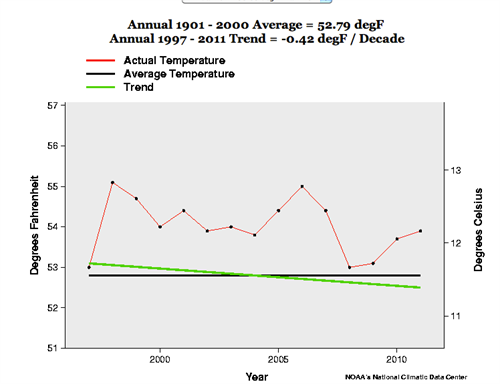
\includegraphics[width=0.5\textwidth]{img/cherry-1.png}
\end{center}
John Coleman, cited by  Anthony Watts, cited by \href{https://tamino.wordpress.com/2013/03/04/cherry-picking-is-childs-play/}{Open Mind}
\end{frame}

\begin{frame}{Not if you zoom out}

\begin{center}
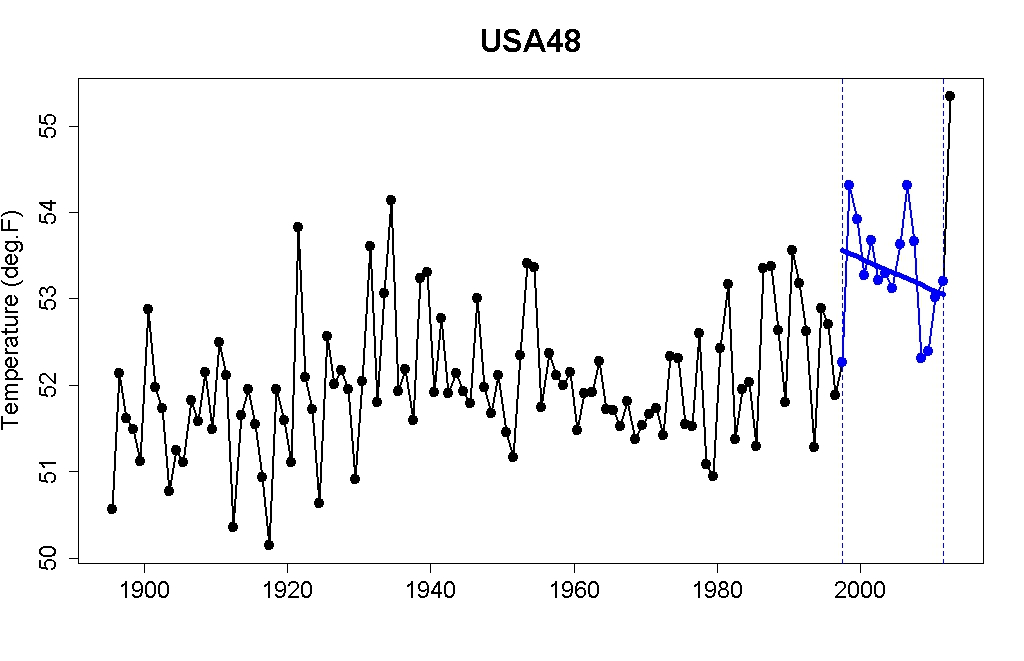
\includegraphics[width=0.6\textwidth]{img/usa48_1.jpg }
\end{center}
\href{https://tamino.wordpress.com/2013/03/04/cherry-picking-is-childs-play/}{Open Mind} \textit{Cherry Picking is Child's Play}
\end{frame}

\begin{frame}{And average over different regions}

\begin{center}
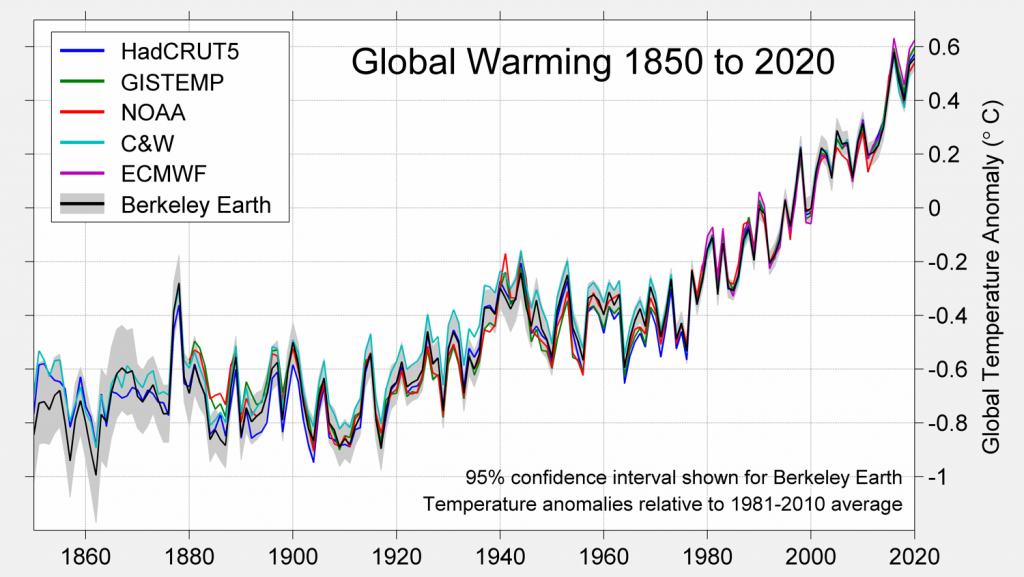
\includegraphics[width=0.6\textwidth]{img/1611534261_comparison-of-global-warming-trend-from-six-different-datasetspng.png}
\end{center}
\href{https://www.climate.gov.ph/news/416}{Climate Change Commission} \textit{CCC: No more time for inaction as global warming accelerates, marking 2020 as one of the warmest years on record}
\end{frame}


% --- CHERRY-PICKING EXAMPLE
\begin{frame}{Example: cherry-picking data}
\textbf{What was done wrong?}
\begin{itemize}
  \item Only the years supporting the argument were shown.  
  \item Broader data contradicts the claimed trend.  
  \item No context or uncertainty provided.
\end{itemize}
\textbf{Better practice:}
\begin{itemize}
  \item Show full dataset and acknowledge anomalies.  
  \item Explain possible causes rather than hiding them.
  \item Show confidence intervals (the grey band in the last image)
  \end{itemize}

 If someone cherry picks data, and refuses to acknowledge it after it has been pointed out, then they are not a credibale source, \ldots
  
\end{frame}

% --- GRAPHICAL DECEPTION
\begin{frame}{How (not) to lie with graphs}
\begin{itemize}
  \item \textbf{Truncated axes} exaggerate small changes.  
  \item \textbf{Omitted error bars} hide uncertainty.  
  \item \textbf{3D charts} distort visual proportions.  
  \item \textbf{Unequal scales} misrepresent relationships.  
\end{itemize}
\begin{center}
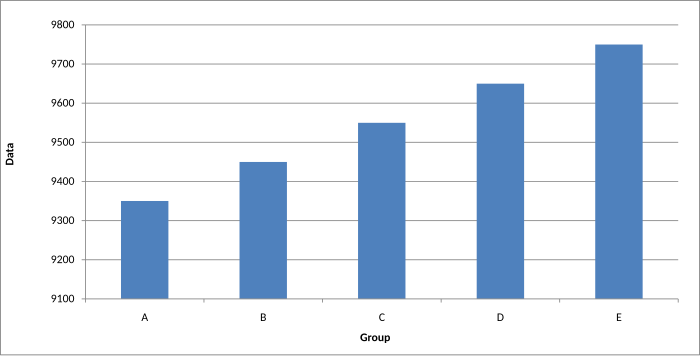
\includegraphics[width=0.4\textwidth]{img/700px-Truncated_Bar_Graph.svg.png} 
\includegraphics[width=0.4\textwidth]{img/700px-Bar_Graph.svg.png} 
\end{center}
Images from \href{https://en.wikipedia.org/wiki/Misleading_graph}{Wikipedia:Misleading graph} (accessed 2025-11-08)
\end{frame}

% --- FROM DATA TO ARGUMENT
\begin{frame}{From data to argument: keeping FAIR and CARE alive}
\begin{itemize}
  \item \textbf{FAIR failures}—missing metadata, unclear methods—lead to weak or unverifiable claims.  
  \item \textbf{CARE failures}—ignoring context or consent—lead to distorted or harmful narratives.  
  \item Ethical writing means:
    \begin{itemize}
      \item Verify data quality and provenance before citing.  
      \item Present uncertainty honestly.  
      \item Represent people and communities with respect.
    \end{itemize}
  \item If we manage data carelessly, our communication cannot be trusted.
  \item This is as true for citing writing as it is for citing data!
\end{itemize}

\end{frame}

% --- CONCLUSION
\begin{frame}{Persuasion with integrity}
\begin{itemize}
  \item Ethical persuasion is clear, evidence-based, and proportionate.  
  \item Data visualisation should illuminate, not impress.  
  \item Sound governance (FAIR/CARE) leads to sound communication.  
  \item Our goal should be \textbf{to inform, not to manipulate.}
\end{itemize}
\end{frame}

% =========================
% When Results Surprise You
% =========================
\section{When Results Surprise You}

% --- INTRODUCTION
\begin{frame}{When what you find  surprises you}
\begin{itemize}
  \item You hypothesised X — but your data support Y, or nothing at all.  
  \item This is not failure — it is how discovery happens.  
  \item Many great findings began as “wrong” results that researchers chose to explore rather than hide.  
  \item Ethical research means reporting what you found, not what you hoped to find.
\end{itemize}
If you discover that what you thought was wrong, \emph{then you have improved your model of the world} --- if you just confirm what you thought, you have gained less!
\end{frame}

% --- ETHICAL RESPONSE
\begin{frame}{Ethical responses to unexpected results}
\begin{itemize}
  \item \textbf{Reflect:} Why might this have happened? Re-examine assumptions, methods, or definitions.  
  \item \textbf{Consider alternatives:} Could sampling, measurement, or confounding factors explain the result?  
  \item \textbf{Report transparently:} Document what changed—methods, data, or interpretation.  
  \item \textbf{Revise hypotheses:} Update theory in light of evidence rather than forcing the evidence to fit theory.  
  \item \textbf{Stay curious:} Unexpected outcomes often open richer questions.
\end{itemize}
\end{frame}

% --- FAIR + CARE CONNECTION
\begin{frame}{FAIR + CARE: supporting honest revision}
\begin{itemize}
  \item \textbf{FAIR} practices—clear metadata, versioning, provenance—let others trace how results emerged.  
  \item \textbf{CARE} principles—context, consent, responsibility—help ensure surprises are interpreted respectfully.  
  \item Keeping complete records allows you (and others) to:  
    \begin{itemize}
      \item Reanalyse the same dataset later.  
      \item Identify methodological errors.  
      \item Learn from data collected by others with proper context.  
    \end{itemize}
  \item This applies to \emph{found data} too: when reusing open datasets, respect their limits and document your reasoning.
\end{itemize}

\end{frame}

% =========================
% Writing Styles: Science, Creativity, Wikipedia
% =========================
\section{Writing for Different Audiences}

% --- COMPARISON OVERVIEW
\begin{frame}{Scientific, creative, and encyclopedic writing}
\begin{itemize}
  \item \textbf{Scientific writing} — formal, objective, structured
    \begin{itemize}
      \item Evidence-based, peer-reviewed, reproducible.  
      \item Goal: to inform and test ideas transparently.
    \end{itemize}
  \item \textbf{Creative writing} — expressive, narrative, open to emotion and metaphor.  
    \begin{itemize}
      \item Goal: to move, provoke, or entertain.  
      \item Truth is emotional or imaginative, not empirical.
    \end{itemize}
  \item \textbf{Wikipedia writing} — concise, neutral, verifiable.  
    \begin{itemize}
      \item Summarises consensus rather than taking sides.  
      \item Accessible to a broad, multilingual audience.
    \end{itemize}
\end{itemize}

\end{frame}

% =========================
% Ethics in Fiction Writing (with citations)
% =========================
\subsection{Ethics in Fiction Writing}

% --- ETHICAL IMAGINATION
\begin{frame}{Ethical imagination}
\begin{itemize}
  \item Fiction gives extraordinary freedom — should there also be responsibility?  
  \item Writers shape how readers see the world, other cultures, and themselves.  
  \item \textbf{Ethical imagination} means using creativity without exploiting others’ pain or identity.  
  \item Ask:
    \begin{itemize}
      \item Whose stories am I telling?  
      \item Do I have the right, or the context, to tell them?  
      \item Who might be harmed or misrepresented by this portrayal?  
    \end{itemize}
  \item Respectful storytelling expands empathy; careless storytelling can reinforce stereotypes or trauma.
\end{itemize}

\medskip
\small Sources: \citep{hachette2021guidediversity, haynes2021ethicsaesthetics, leclerc2024writing}
\end{frame}

% --- CULTURAL SENSITIVITY AND RESPONSIBILITY
\begin{frame}{Cultural sensitivity and responsibility}
\begin{itemize}
  \item \textbf{Cultural sensitivity} is not censorship — it is awareness.  
  \item Portray groups and traditions accurately, based on research and listening.  
  \item Avoid:
    \begin{itemize}
      \item Using cultural elements as exotic decoration (“appropriation”).  
      \item Reducing people to symbols or stereotypes.  
      \item Borrowing trauma without accountability.  
    \end{itemize}
  \item When writing outside your own experience:
    \begin{itemize}
      \item Consult people from that background.  
      \item Be open to feedback and revision.  
      \item Prioritise authenticity over authority.
    \end{itemize}
  \item Ethical fiction balances creative freedom with empathy and respect for real lives.
\end{itemize}
\medskip
\small Sources: \citep{ocallaghan2025culturalsensitivity, maguire2009ethicsfiction, hachette2021guidediversity}

\begin{center}
\emph{I am not an expert here}  
\end{center}

\end{frame}



% =========================
% Transition to Discussion / Activity
% =========================
\section{Practice!}

\begin{frame}{Auditing sources for FAIR and CARE issues}
\begin{itemize}
  \item Next, we’ll spend about \textbf{30 minutes} discussing and practising what we’ve learned.  
  \item Two connected parts:
    \begin{enumerate}
      \item \textbf{Discussion of last week’s annotated bibliography.}  
            Share one source you found insightful or problematic.  
      \item \textbf{Source audit activity.}  
            Choose one of your sources and check:
            \begin{itemize}
              \item Is it \textbf{Findable, Accessible, Interoperable, Reusable}?  
              \item Does it respect \textbf{Collective Benefit, Authority to Control, Responsibility, Ethics}?  
            \end{itemize}
    \end{enumerate}
  \item Work individually or in pairs; we’ll share highlights at the end.
\end{itemize}
\textit{Our goal: to read sources not only for what they say, but for how responsibly they were created.}
\end{frame}

% --- STUDENT ASSIGNMENT CONTEXT
\begin{frame}{Your first-draft paper: fitting the scientific style}
\begin{itemize}
\item The upcoming assignment is your \textbf{first draft of a short academic paper.}
 
  \item Use the conventions of scientific writing:
    \begin{itemize}
      \item Clear research question and motivation.  
      \item Evidence-based argument supported by credible sources.  
      \item Neutral tone; cautious interpretation; accurate citations.
    \end{itemize}
  \item Your annotated bibliography and Wikipedia writing experience both help:
    \begin{itemize}
      \item Bibliography → evaluating sources and citation style.  
      \item Wikipedia → writing neutrally and clearly for others.
    \end{itemize}
\end{itemize}

I want to see how well you can use your sources to answer the question, as accurately as possible.

\begin{itemize}
\item Next week, you will read each others papers and comment on them.
\end{itemize}

\end{frame}

% =====================================================================

\begin{frame}{Acknowledgements}

  \begin{itemize} %%%FIXME --- REDO
  \item \textcite{openai-chatgpt-2025-03-14} was used to format the references, and generate a first draft of the slides
  \end{itemize}
  
\end{frame}



\section{References}
% =====================================================================
\begin{frame}[allowframebreaks]
\frametitle{References}
\printbibliography[heading=none]
\end{frame}

\end{document}
%%% Local Variables: 
%%% coding: utf-8
%%% mode: latex
%%% TeX-PDF-mode: t
%%% TeX-engine: luatex
%%% End: 

